\documentclass[t]{beamer}
\usetheme{Copenhagen}
\setbeamertemplate{headline}{} % remove toc from headers
\beamertemplatenavigationsymbolsempty

\usepackage{amsmath, array, tikz, bm, pgfplots, tcolorbox, graphicx, venndiagram, color, colortbl, xfrac}
\pgfplotsset{compat = 1.16}
\usepgfplotslibrary{statistics}
\usetikzlibrary{calc}

\title{Scatterplots and Correlation}
\author{}
\date{}

\AtBeginSection[]
{
  \begin{frame}
    \frametitle{Objectives}
    \tableofcontents[currentsection]
  \end{frame}
}

\begin{document}

\begin{frame} 
\maketitle
\end{frame}

% Create scatterplots
\section{Create and analyze scatterplots}

\begin{frame}{Scatterplots}
\begin{tcolorbox}[colframe=green!20!black, colback = green!30!white,title=\textbf{Scatterplot}]
A \textbf{scatterplot} is a visual display which can be used to examine an association between two variables, usually $x$ and $y$.
\end{tcolorbox}
\bigskip	\pause

The independent variable, $x$, is called the {\color{blue}\textbf{explanatory variable}} and the dependent variable, $y$, is called the {\color{blue}\textbf{response variable}}.	\bigskip	\pause

Scatterplots allow us to see if there is a relationship between the two variables.
\end{frame}

\begin{frame}{Example 1}
The table below shows the age of a certain model of car (in years) with the cars current value (in thousands of dollars). Create a scatterplot for the data.	\newline\\
\begin{minipage}{0.3\textwidth}
\scalebox{0.9}{
\begin{tabular}{c|c}
\textbf{Age} & \textbf{Value} \\ \hline
2 & 15 	\\
3 & 12	\\
3 & 13	\\
2 & 14	\\
4 & 13	\\
5 & 10	\\
6 & 10.5	\\
1 & 16.5	\\
0 & 18		\\
4 & 14		\\
7 & 11		\\
\end{tabular}}
\end{minipage}
\hspace{0.25cm}
\onslide<2->{
\begin{minipage}{0.6\textwidth}
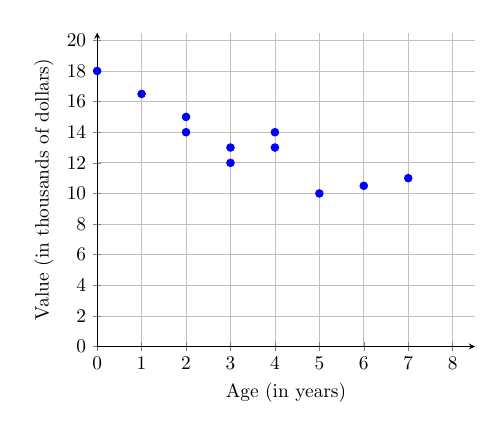
\begin{tikzpicture}[scale=0.7]
	\begin{axis}[
	axis lines = left, grid,
	xlabel = {Age (in years)},
	ylabel = {Value (in thousands of dollars)},
	xmin = 0, xmax = 8.5,
	ymin = 0, ymax = 20.5,
	xtick = {0,1,...,8},
	ytick = {0,2,...,20}
	]
	\addplot [only marks, color=blue] coordinates {
		(2,15)
		(3,12)
		(3,13)
		(2,14)
		(4,13)
		(5,10)
		(6,10.5)
		(1,16.5)
		(0,18)
		(4,14)
		(7,11)
	};
	\end{axis}
\end{tikzpicture}
\end{minipage}}
\end{frame}

\section{Determine the type of correlation of a scatterplot}

\begin{frame}{Direction of Points}
Often times, the data in a scatterplot has some pattern to it. \newline\\	\pause

\begin{tcolorbox}[colframe=green!20!black, colback = green!30!white,title=\textbf{Correlation}]
A \textbf{correlation} between two variables examines how the response variable's ($y$) values change as the explanatory variable's ($x$) values change.
\end{tcolorbox}
\bigskip \pause

We will examine three correlation types: positive, negative, and none (a.k.a. no correlation)
\end{frame}

\begin{frame}{Positive Correlation}
As $x$ increases, so does $y$.	\newline\\	\pause
\begin{center}
\begin{tikzpicture}[scale=0.7]

\end{tikzpicture}
\end{center}
\end{frame}
% Examine mean(x) and mean(y) and correlation

\end{document}